\documentclass[11pt]{article}
\title{Will's Adventures with MapReduce}
\author{Will Ware \texttt{<wware@alum.mit.edu>}}
\date{}

% PDFLaTeX Support
\newif\ifpdf
\ifx\pdfoutput\undefined
   \pdffalse
\else
   \pdfoutput 1
   \pdftrue
\fi

\usepackage{makeidx}

\topmargin=-.75in
\oddsidemargin=0in
\evensidemargin=0in
\textwidth=6.5in
\textheight=9.5in

% Hypertext links
\ifpdf
   \usepackage[
     pdftex,
     pdftitle={Micro Driver APIs and Overview},
     pdfsubject={},
     pdfauthor={Will Ware},
     pdfstartview={FitH},
     bookmarks=true,
     bookmarksopen=false,
     colorlinks=true
   ]{hyperref}
\fi

\ifpdf
  \usepackage[pdftex]{graphicx}
  \pdfcompresslevel=9
  \DeclareGraphicsExtensions{.jpg,.pdf,.mps,.png}
  \graphicspath{{PDF/}}
\else
  \usepackage{graphicx}
  \usepackage[dvips]{graphicx}
  \DeclareGraphicsExtensions{.eps,.ps,.bmp,.tif,.tiff,.tga}
  \graphicspath{{EPS/}}
\fi

\makeindex

\begin{document}

\thispagestyle{plain}
\pagenumbering{roman}
\maketitle

\tableofcontents
\pagenumbering{arabic}

\section{What is MapReduce all about?}

MapReduce has become a widely-used de-facto standard for a large class
of distributed computations. Google uses it internally for thousands
of different tasks. It has been embraced by many other organizations.
It is well studied and there are implementations for a lot of
different hardware and network platforms.

\begin{figure}
\begin{center}
\includegraphics[width=6in]{mr_arch.pdf}
\end{center}
\caption{The MapReduce architecture}
\label{F:architecture}
\end{figure}

As we start to reach the end of Moore's Law, multi-core processors and
distributed computing will be the only way to get more speed. Anything
useful in that vein becomes compellingly interesting.

So a facility with MapReduce can translate to continuing relevance in
today's job market, and may also be a prerequisite for deeply
understanding computer science as we go forward.

\subsection{Instructional material}

Here's a five-part video course that Google offers for grokking MapReduce.

\begin{itemize}
\item{\tt http://www.youtube.com/watch?v=yjPBkvYh-ss} \\ Lecture 1, Distributed computing background
\item{\tt http://www.youtube.com/watch?v=-vD6PUdf3Js} \\ Lecture 2, MapReduce origins and basics
\item{\tt http://www.youtube.com/watch?v=5Eib\_H\_zCEY} \\ Lecture 3
\item{\tt http://www.youtube.com/watch?v=1ZDybXl212Q} \\ Lecture 4
\item{\tt http://www.youtube.com/watch?v=BT-piFBP4fE} \\ Lecture 5
\end{itemize}

UCBerkeley lectures on MapReduce, from CS 61A
\begin{itemize}
\item {\tt http://www.youtube.com/watch?v=mVXpvsdeuKU} \\ Lecture 34
\item {\tt http://www.youtube.com/watch?v=NjAKl5B0BKs} \\ Lecture 35
\end{itemize}

Other stuff
\begin{itemize}
\item {\tt http://developer.yahoo.com/hadoop/tutorial/index.html}
  \\ Yahoo Hadoop Tutorial
\item {\tt
  http://hadoop.apache.org/core/docs/current/hdfs\_design.html}
  \\ HDFS Architecture
\item {\tt http://michaelnielsen.org/blog/?p=529} \\ An
  intelligent-looking blog post
\item {\tt http://michaelnielsen.org/blog/?cat=57} \\ A whole bunch
  of very intelligent-looking blog posts by the same guy
\item {\tt http://michaelnielsen.org/blog/?page\_id=503} \\ an index
  of blog posts on the Google Technology Stack
\end{itemize}
Google's internal MapReduce implementation takes into account the
possibility of hardware failure. Evidently they don't throw away any
results from GFS until they're certain that piece has been computed.
So all the intermediate stuff stays around until all the reduce jobs
are all done.

\subsection{Things that initially confused me}

Initially, I didn't quite get the way Google framed the reduce
function. By comparison with reduction in Lisp or Scheme, I had
expected

\begin{verbatim}
reduce : (v2, list(v2)) -> list(v2)
\end{verbatim}

but instead they have

\begin{verbatim}
reduce : (k2, list(v2)) -> list(v2)
\end{verbatim}

This takes k2 into account and may therefore be more general.
Interesting, the reduce job for a particular k2 is NOT parallelizable,
because v2 values must be processed in order. Reduces for different
k2s can be parallelized but for a particular k2, the reduce is
inherently serial.

Frequently, the reduce function will ignore its k2 argument.

\subsection{Thinking in MapReduce terms}

There are a few principles that seem to guide MapReduce that appear to
represent a big change in how we think about distributed computing.
\begin{itemize}
\item The most efficient way to use hard drives is with big streaming
  reads.
\item The machines in a cluster should be anonymous from the POV of
  the app developer. His code should never address an individual
  machine, it should only describe what is to be done, and the
  infrastructure should do the rest.
\item In big enough clusters, hardware failures will be frequent and
  inevitable.
\item {\tt http://www.cloudera.com/hadoop-training-thinking-at-scale}
  \\ go through this and take notes
\end{itemize}

\subsection{Iterators in MapReduce}

The bigger deal here is the representation of ``list(v2)''. The MR
paper glibly says \index{iterator}``an iterator'', but this iterator
hides the question of whether the list is small enough to fit in
memory, or big enough to need to live on the hard disk, or possibly
many hard disks.

The iterator is a crucial part of the design of the distributed file
system. The iterator needs to know that v2 values for a particular k2
are interleaved across several workers, and must be kept in order.
Java's Iterator interface is read-only, but you need a writable
version to which you can append stuff. When you create an instance of
the iterator, it starts out empty.

I want to give a good bit of thought to the iterator that feeds the
reduce function. The v2 values for a particular k2 key will be spread
across machines in a sort of run-length-encodable way. So for k2=3,
you might have five v2 values on Alpha, then 15 on Beta, then three
more on Alpha, then six on Gamma. The iterator needs to keep track
of all that, and know where to find each v2 entry wherever it may be.
So the iterator is equivalent to a linked list where each link has a
pointer to a machine, a pointer to a v2 value on that machine, and the
size of that v2 value in bytes. The iterator itself is not very big
and can be passed around the network pretty easily.

What does Python's iterator API look like to the user writing the
reduce function? \\ {\tt
  http://docs.python.org/library/stdtypes.html\#iterator-types}
\\ It's pretty darn simple, and it automatically fits into Python's
``for x in lst'' syntax.

Permit v2 values to be potentially large, e.g. uncompressed HD movie
frames. My thought is to store them on the hard disk in files that are
no smaller than 1 megabyte, something you can easily pull into memory.

My iterator needs to be able to handle appends also. Actually, maybe
not: the MR paper specifies EmitIntermediate and Emit functions. That
means, put the key-value pair in some future iterator for which you
don't now have read access. The iterator you're reading is
non-writable.

The input stream that feeds the map operators should ALSO be an
iterator, though it probably wants some extra magic methods so that it
can grab a block from the middle of the iterator, which the normal one
can't do. Maybe it should be able to do it? Maybe you'd have list
slices, which can also have their own iterators?

It's critical to get the v2 values in the right order for each k2, and
they may be computed out of order. So you'll need to stitch together
linked lists into a big one, and keep track of the k1 index for each
small linked list. Lists must be doubly linked for quick append.

Think of each k2 as a channel of debug spew, and on a serial machine
the map jobs would always run sequentially and never overlap in time,
so that gives you the order that v2s need to come in, and you can
write tests on that basis for testing distributed implementations.
Meanwhile people can test their code on serial machines, confident
that the distributed implementation will give the same v2 ordering.

\section{Hadoop and Happy}

Apache Hadoop Core is a software platform that lets one easily write
and run applications that process vast amounts of data. Here's what
makes Hadoop especially useful:
\begin{itemize}
\item Scalable: Hadoop can reliably store and process petabytes.
\item Economical: It distributes the data and processing across clusters of commonly available computers. These clusters can number into the thousands of nodes.
\item Efficient: By distributing the data, Hadoop can process it in parallel on the nodes where the data is located. This makes it extremely rapid.
\item Reliable: Hadoop automatically maintains multiple copies of data and automatically redeploys computing tasks based on failures.
\end{itemize}
Hadoop implements MapReduce, using the Hadoop Distributed File System
(HDFS). MapReduce divides applications into many small blocks of work.
HDFS creates multiple replicas of data blocks for reliability, placing
them on compute nodes around the cluster. MapReduce can then process
the data where it is located.

\begin{figure}
\begin{center}
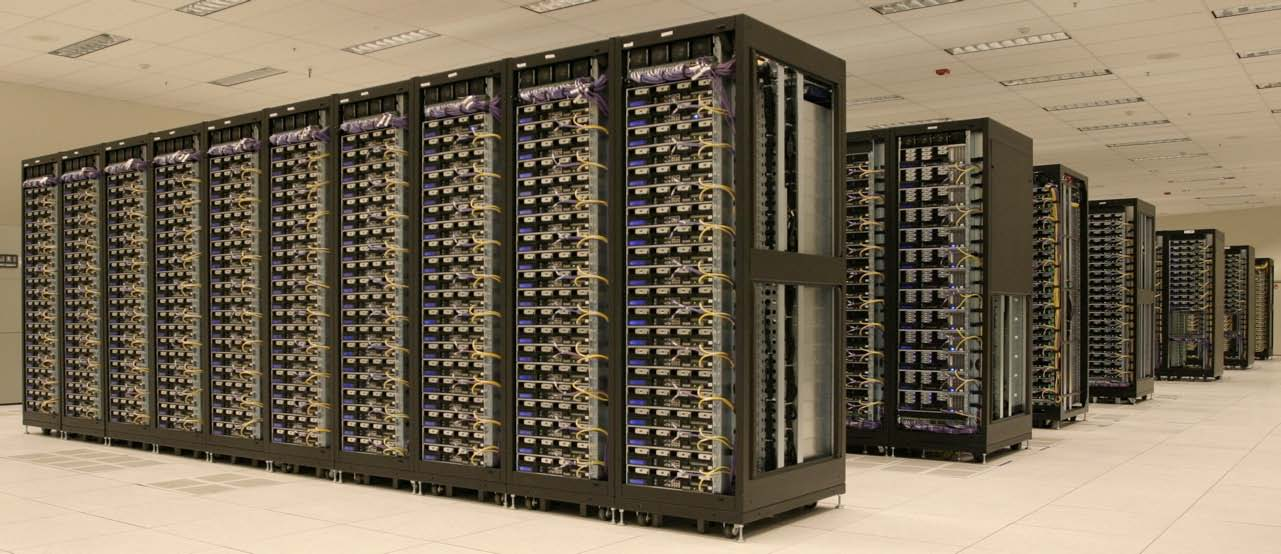
\includegraphics[width=6in]{Yahoo-hadoop-cluster.pdf}
\end{center}
\caption{Yahoo runs Hadoop on this large cluster}
\label{F:hadoopcluster}
\end{figure}

Hadoop has been demonstrated on clusters with 2000 nodes. The current
design target is 10,000 node clusters.

\subsection{Happy}

Happy is a framework for writing map-reduce programs for Hadoop using
Jython. It files off the sharp edges on Hadoop and makes writing
map-reduce programs a breeze.

{\tt http://code.google.com/p/happy/}

\subsection{Should I use Hadoop?}

Why not use Hadoop? Why yet another MapReduce implementation? Why
Python? There are numerical packages for Java at \\ {\tt
http://math.nist.gov/javanumerics/} \\ so the lack of numpy isn't a
problem. For native executables, Java provides java.lang.Runtime with
some exec() methods.

Hadoop is designed for large clusters with multiple racks of machines.
My thing can be for people who have only three or four machines
available, and who just want to learn about MapReduce without a big
investment. Maybe it makes sense to try to run Hadoop on a small
cluster, and assume it works until it visibly fails.

Rolling my own would keep it small and simple, and I'd document it
thoroughly, to show how it was put together and what all the reasoning
was. Hadoop is presented as a fait accompli, and those design
decisions aren't well documented.

Maybe the idea then would be to document Hadoop deeply in the same
way, discussing all the design decisions. So this is really a
write-a-book project, not a write-software project.

O'Reilly has a Hadoop book coming out in July 2009, see \\ {\tt
  http://oreilly.com/catalog/9780596521998/} \\ Is it sane to try to
write my own? Typically the O'Reilly book will discuss installation
and examples, but it might not dig deeply into design decisions.

A big motivation here is to pave the way for future employment,
possibly at Google, possibly elsewhere. This will require showing deep
insight into MapReduce implementation vibes. For this purpose, the
inquiry into design decisions is crucially important.

I go back and forth about whether to use Hadoop/Happy or roll my own.
Right now I'm leaning toward rolling my own at least initially. It
would be a good learning experience, and it could be helpful for
people who don't want to tackle Hadoop.

The danger of simply bringing up Hadoop on a small cluster is that I'm
not forcing myself to dig deep into the design issues. Besides,
another implementation might bring something new to the table that
Hadoop doesn't offer. A pure-Python MR implementation would make the
Python community happy, and that would be another place where I could
build professional connections.

Think about a unit-testing strategy for a MapReduce implementation. It
should be pretty quick to put together, the keys and values can all be
integers. So the run time should also be very short. First get the
test working in the serial case.

Then write a parallel implementation using multiple processes on a
single machine. Make sure the test still passes. You won't need a
distributed filesystem for that.

Start writing tests that deal with larger data sets. Eventually it
will force the issue of writing a distributed filesystem, or at least
thinking carefully about how to build queues.

The alternative to this is to fool with Hadoop. I wonder if I can
bring up Hadoop in single-cpu mode on a Windows laptop.

Writing tests and examples for Hadoop isn't the worst thing I could
ever work on.

\subsection{Amazon's Hadoop-for-rent cluster}

{\tt http://aws.amazon.com/elasticmapreduce/}

The price for MapReduce services on Amazon appears pretty cheap, but
there's a lot I don't know. Is it running on Linux machines? What
languages are allowed? How do I get my code onto their cluster?

Amazon Elastic MapReduce allows you to implement data processing
applications in many languages including Java, Perl, Ruby, Python,
PHP, R, or C++. You can test these applications on different instance
types and job flow sizes to pick the optimal performance settings for
your specific case.

This would be a good thing to try. Think of several examples to test
on AEMR, having developed them with my own Python code and found them
untenably large for a sequential single-CPU machine.

\section{Rolling my own implementation}

This is a useful thought exercise even if I never actually do it.

\subsection{Hardware}

The question arises of how to build a cluster inexpensively. There are
two sources of cheap computers that I can think of. One is places like
eBay and Craigslist. The other is computer recycling outfits, which
service businesses that are unloading their old computers. The
recyclers make most of their money by providing data erasure services,
so hopefully the erased hardware is pretty cheap.

I have three machines at home I can use. Why not just do that? Why
bother getting a bunch of new machines? If anything, the valuable
thing to do would be to update the hard drives.

\subsection{Design considerations}

When the controller wants to send a job to a map worker, it sends a
block of (k1,v1) pairs to it. The TCP connection stays up until that
map job is complete. The response from the map worker is the histogram
of k2 values for that job, and the controller has the task of keeping
track of which worker has which k2 values and how many of them, which
enables the controller to schedule reduce jobs with minimal
communication overhead.

Actually, the controller {\em doesn't} need to do that.

Do I need to sort the (k2,v2) values for a particular k2 value? No - I
need to preserve the order in which they were {\em generated}. So think
about how to do that. Within the block of (k2,v2) from ealready be
sorted, so just get those blocks in the right order.

The reduce job is a k2 value and a list of block indices, presented in
the correct order. The HTTP response of the reduce job is the the v2
set for that k2.

\subsection{Hashspace}

Use my old LinuxTuples code as the comm infrastructure for MapReduce.
Add a uniqueID type, which is a 128-bit integer generated using {\tt
  /dev/urandom}. Distribute the tuplespace among all the machines.
Think about queues and k2 locality and how to distribute reduce jobs
wisely.

Replace tuples with hashtables, essentially Python dictionaries with
strings as keys, and the values are arbitrary byte strings. Think
about how matching would work in that case, what templates look like,
how to make matching efficient while taking into account the network
topology.

When thinking about distributing the hashtable space, think about
handling gigabyte hashtables. Think about nearness metrics and how to
support them under the covers. Think about something like this: if I'm
a machine looking for a job, I need to favor the jobs whose inputs are
mostly local on my own hard disk. Only move data across the network
when really necessary.

I'm going to need a cluster simulator that does run-length-encoded
time just like those digital logic simulators. So compute time and
communication time need to be in there. When that simulator is ready
(which should be easy) then I can start working up the algorithms for
matching and nearness metrics, and ways to choose jobs smartly.

I did a teeny bit of work on the cluster sim, just the event stuff.
Events in Python are quick, that's good. Network overhead is
represented by two NxN symmetric matrices with zero diagonals to form
An+B for an n-byte message. Matrices can be derived empirically and I
can start with a teeny 3-machine cluster.

The hashtable space is distributed, templates are just hashtables with
fewer keys, but maybe with some way to be identifiable as a template.
Each machine runs a tcp server, and given a template, can provide info
about what matches it has and their sizes. This is sused by a worker
looking for a job so he can favor job that minimize comm overhead.

So the hashspace is a space where you can PUT, GET, or READ a
hashtable just as you can do with tuples in a tuples space. It's
trivial to implement other spaces (distributed filesystem, tuple
space) on top of a hashspace. Each hashtable is a Python dictionary
where the keys are (relatively short) byte sequences and the values
are potentially large byte sequences. Keys are typically interpreted
as ASCII strings but could alternatively be taken as long integers.

A full reference implementation for a hashspace can be done nicely in
Python. Treat each hashtable as a dictionary and use pickle or cPickle
for serialization. There may not be any need to move to C or C++,
we'll see about that.

Note that there can be multiple identical hashtables floating around
in the space.

A query is where one machine passes another a template and the second
guy passes back the list of lengths for matching hashtables.

One thing you need is to handle different kinds of linked lists of
hashtables. The forward link on a hashtable is of the form {\tt next:
  8914701238740}, where the value is a unique ID so the next hashtable
in the list has {\tt uid: 8914701238740}. In particular, the results
of reduce operations will consist of linked lists of linked lists, so
along the spine, each guy has a ``child'' in addition to a ``next''.
When I'm a worker looking for a reduce job with minimal comm overhead,
I want to traverse both dimensions to get the complete cost (some of
that is farmed out to the other machines hosting some of those
things).

\subsection{Hashspace locking for atomic operations}

One locks the hashspace by calling a lock function with a template for
the hashtables to be locked. On the local machine, the system looks to
see if there are (a) any conflicting locks already present or (b) any
non-overlapping locks.

The problem with non-overlapping locks is that they make it possible
for a hashtable to be locked by one but not the other, or to be locked
by both, and those choices are independent. So a lot of thought is
needed there to think about every possible scenario. It may be
necessary to throw an exception if you try to lock against a
non-overlapping lock.

If there is already a conflicting lock present, then the lock function
needs to block until that lock is gone. This is just the same behavior
as you'd see with ``synchronized'' in Java or ``lock'' in C\#. The app
sees it as blocked, but what really happens is that it relinquishes
the lock, waits some small amount of time, and retries.

Once the lock is established on the local machine, it tries to lock
all the other machines with the same template. Any failure to do so
means that it relinquishes all locks, waits a while, and tries again.

The unit tests for locking need to include the following scenarios.
\begin{itemize}
\item Establish a lock and make sure that GET and PUT block.
\item Have two machines try conflicting locks at the same time. Make
  sure that only one wins, and when he relinquishes, the other guy
  gets to go.
\end{itemize}
I'm sure there are others but that's what comes right to mind.

So the API for the hashspace has locking and relinquishing as basic
operations, at a level below GET and PUT. It might make sense to come
up with a new collection of primitives.

\section{Doing stuff with HDFS, other random thoughts}

Even if I don't want to use Hadoop, I should still be thinking hard
about using HDFS. Many interesting things could be built on top of it.
Certainly the hashspace could be done that way.

For problems that can't be done with MapReduce, you can define
dependency graphs where the vertices are data sets and the edges are
programs to be run. Use HDFS to store the data and write an
infrastructure that reasonably distributes the execution of programs.
Think up a concise painless syntax for building large dependency
graphs, and implement it in Python. Think about how to assign tasks,
bearing in mind the locality of the data and the possibility of
hardware failures.

Each vertex in the graph has a version number, and you hang on to the
last few versions, whatever you need to ensure that you won't lose
anything if an individual machine crashes.

\printindex

\end{document}
